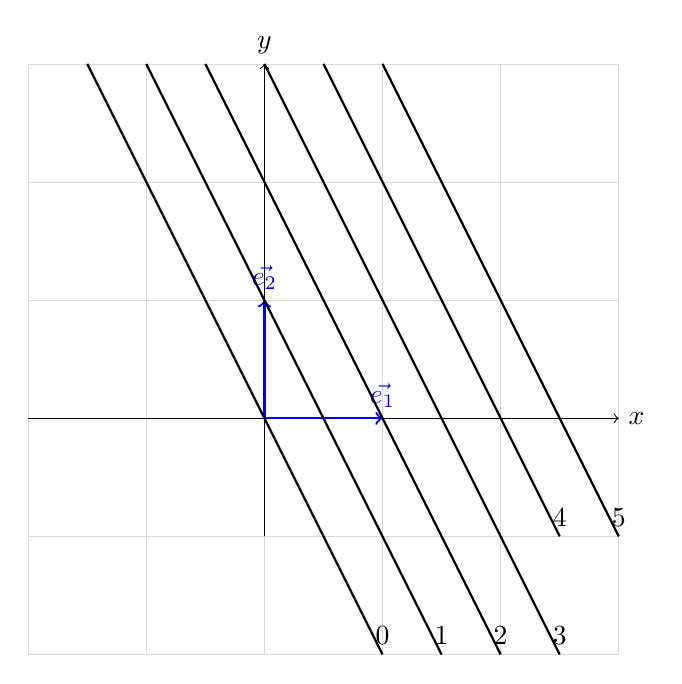
\begin{tikzpicture}[scale=1.5]
  \draw[step=1cm,gray!30,very thin] (-2,-2) grid (3,3);
  \draw[->] (-2,0) -- (3,0) node[right] {$x$};
  \draw[->] (0,-1) -- (0,3) node[above] {$y$};
  \draw[->,thick,blue] (0,0) -- (1,0) node[above] {$\vec{e_1}$};
  \draw[->,thick,blue] (0,0) -- (0,1) node[above] {$\vec{e_2}$};
  \draw[black,thick,domain=-1.5:1] plot (\x,{-2*\x}) node[above] {0};
  \draw[black,thick,domain=-1:1.5] plot (\x,{-2*\x+1}) node[above] {1};
  \draw[black,thick,domain=-0.5:2] plot (\x,{-2*\x+2}) node[above] {2};
  \draw[black,thick,domain=0:2.5] plot (\x,{-2*\x+3}) node[above] {3};
  \draw[black,thick,domain=0.5:2.5] plot (\x,{-2*\x+4}) node[above] {4};
  \draw[black,thick,domain=1:3] plot (\x,{-2*\x+5}) node[above] {5};
\end{tikzpicture}
